\section{Fundamental results from Fourier analysis} \label{app::Fourier}
In this appendix, we state several fundamental results from Fourier analysis for doubly periodic functions, associated with the Fourier transform pair defined in Definition~\ref{Def::Fourier}. These results are useful for us, and their proofs are well established and can be referenced in classical literature, such as in the work of Stein and Shakarchi~\cite{stein2011fourier}.
\begin{lem}\label{lem::Convolution}
	(Convolution theorem) Let $f(\bm{\rho},z)$ and $g(\bm{\rho},z)$ be two functions which are periodic in $\bm{\rho}$ and non-periodic in $z$. Suppose that $f$ and $g$ have Fourier transform $\widetilde{f}$ and $\widetilde{g}$, respectively. Their convolution is defined by
	\begin{equation}\label{eq:Q2D_cov}
		u(\bm{\rho},z):=(f\ast g)(\bm{\rho},z)=\int_{\mathcal{R}^2}\int_{\mathbb{R}}f(\bm{\rho}-\bm{\rho}',z-z')g(\bm{\rho}',z')dz'd\bm{\rho}',
	\end{equation}
	satisfying
	\begin{equation}
		\widetilde{u}(\bm{k},\kappa)=\widetilde{f}(\bm{k},\kappa)\widetilde{g}(\bm{k},\kappa).
	\end{equation}
	
\end{lem}
\begin{lem}\label{lem::Poisson}
	(Poisson summation formula) Let $f(\bm{\rho},z)$ be a function which is periodic in $\bm{\rho}$ and non-periodic in $z$. Suppose that $f$ has Fourier transform $\widetilde{f}$ and $\bm{r}=(\bm{\rho},z)$. Then one has
	\begin{equation}
		\sum_{\bm{m}\in \mathbb{Z}^2} f(\bm{r} + \V{\mathcal{M}}) = \frac{1}{2\pi L_x L_y}\sum_{\bm{k}\in \mathcal{K}^2}\int_{\mathbb{R}}\widetilde{f}(\bm{k},\kappa)e^{\m{i} \bm{k}\cdot\bm{\rho}}e^{\m{i} \kappa z}d\kappa.
	\end{equation}
\end{lem}
\begin{lem}\label{lem::2dfourier}
	(Radially symmetric functions) 
	Suppose that $f(\rho,z)$ is periodic and radially symmetric in $\bm{\rho}$, i.e., $f(\bm{\rho},z)=f(\rho,z)$. Then its Fourier transform $\widetilde{f}$ is also radially symmetric. Indeed, one has
	\begin{equation}
		\widetilde{f}(\rho,z)=2\pi\int_{0}^{\infty}J_0(k\rho)f(\rho,z)\rho d\rho.
	\end{equation}
\end{lem}

% \gao{remove the Appendix A `Derivation of Ewald2D method'}

\section{Proof of Lemma~\ref{thm::SpectralExpansion}}\label{app::deriv}
By applying the Fourier transform to Poisson's equation
\begin{equation}\label{eq::B.1}
	-\Delta\phi_{\ell}(\bm{\rho},z)=4\pi g(\bm{\rho},z)\ast\tau(\bm{\rho},z),
\end{equation}
one obtains  
\begin{equation}\label{eq::B2}
	\widetilde{\phi}_{\ell}(\bm{k},\kappa)=\frac{4\pi}{k^2+\kappa^2}\widetilde{g}(\bm{k},\kappa)\widetilde{\tau}(\bm{k},\kappa)\quad\text{with}\quad \widetilde{g}(\bm{k},\kappa)=\sum_{j=1}^{N}q_{j} e^{-\m{i} \bm{k}\cdot\bm{\rho}_{j}}e^{-\m{i} \kappa z_{j}}
\end{equation}
via the convolution theorem and the Poisson summation formula (see Lemmas~\ref{lem::Convolution} and \ref{lem::Poisson}, respectively). Applying the inverse Fourier transform to Eq.~\eqref{eq::B2} yields
\begin{equation}\label{eq::phil}
	\phi_{\ell}(\bm{\rho},z)=\frac{2}{L_xL_y}\sum_{j=1}^{N}q_{j}\sum_{\bm{k}\neq\bm{0}}\int_{\mathbb{R}}\frac{e^{-(k^2+\kappa^2)/(4\alpha^2)}}{k^2+\kappa^2}e^{-\m{i} \bm{k}\cdot(\bm{\rho}-\bm{\rho}_{j})}e^{-\m{i} \kappa(z-z_{j})}d\kappa + \phi^{\bm{0}}_{\ell}(z),
\end{equation}
where $\phi^{\bm{0}}_{\ell}(z)$ is the contribution from zero mode. From \cite{oberhettinger2012tables}, one has 
\begin{equation}\label{eq::integral}
	\int_{\mathbb{R}} \frac{e^{-(k^2+\kappa^2)/(4\alpha^2)}}{k^2+\kappa^2} e^{-\m{i} \kappa z} d\kappa = \frac{\pi}{2k} \left[\xi^{+}(k,z)+\xi^{-}(k,z)\right]
\end{equation}
for $\bm{k}\neq\bm{0}$, where $\xi^{\pm}(k,z)$ are defined via Eq.~\eqref{eq::xi20}. Substituting Eq.~\eqref{eq::integral} into the first term of Eq.~\eqref{eq::phil} yields $\phi_{\ell}^{\bm{k}}(\bm{r})$ defined via Eq.~\eqref{eq:philk}.

By Theorem~\ref{order}, the zero-frequency term $\phi^{\bm{0}}_{\ell}(z)$ always exists and its derivation is very subtle. Let us apply the 2D Fourier transform (see Lemma~\ref{lem::2dfourier}) to Poisson's equation Eq.~\eqref{eq::B.1} only on periodic dimensions, and then obtain
\begin{equation}\label{eq::B.5}
	(-\partial_z^2+k^2)\widehat{\phi}_{\ell}(\bm{k},z)=4\pi\widehat{g}(\bm{k},z)\ast_{z}\widehat{\tau}(\bm{k},z),
\end{equation}
where $\ast_z$ indicates the convolution operator along $z$ dimension. Simple calculations suggest
\begin{equation}
	\widehat{g}(\bm{k},z)=\sum_{j=1}^{N}q_{j} e^{-\m{i} \bm{k}\cdot\bm{\rho}_{j}}\delta(z-z_{j}),\quad\text{and}\quad \widehat{\tau}(\bm{k},z)=\frac{\alpha}{\sqrt{\pi}} e^{-k^2/(4\alpha^2)}e^{-\alpha^2z^2}.
\end{equation}
The solution of Eq.~\eqref{eq::B.5} for $\bm{k}=\bm{0}$ can be written as the form of double integral that is only correct up to a linear mode,
\begin{equation}\begin{split}
		\phi_{\ell}^{\bm{0}}(z)&=-\frac{4\pi}{L_xL_y}\int_{-\infty}^{z}\int_{-\infty}^{z_1}\widehat{g}(\bm{0},z_2)\ast_{z_2}\widehat{\tau}(\bm{0},z_2)dz_2dz_1+A_0z+B_0\\
		&=-\frac{2\pi}{L_xL_y}\sum_{j=1}^{N}q_{j}\left[z-z_{j}+(z-z_{j})\erf\left(\alpha(z-z_{j})\right)+\frac{e^{-\alpha^2(z-z_{j})^2}}{\sqrt{\pi}\alpha}\right]+A_0z+B_0.
	\end{split}
\end{equation}
To analyze the short-range component $\phi_{s}(\bm{\rho},z)$ using a procedure similar to Eqs.~\eqref{eq::B.1}-\eqref{eq::integral}, one obtains
\begin{equation}\begin{split}
		\phi_{s}^{\bm{0}}(z) =& \frac{\pi}{L_x L_y} \sum_{j=1}^{N} \lim_{\bm{k}\rightarrow\bm{0}} \frac{1}{k} \left[2e^{-k|z|}-\xi^{+}(\bm{k},z) - \xi^{-}(\bm{k},z)\right]\\
		=& \frac{2\pi}{L_xL_y}\sum_{j=1}^{N}q_{j}\left[-|z-z_{j}|+(z-z_{j})\erf\left(\alpha(z-z_{j})\right)+\frac{e^{-\alpha^2(z-z_{j})^2}}{\sqrt{\pi}\alpha}\right].
	\end{split}
\end{equation}
Since $\phi_{s}^{\bm{0}}(z)+\phi_{\ell}^{\bm{0}}(z)$ matches the boundary condition Eq.~\eqref{eq::boundary1} as $z\rightarrow \pm\infty$ and by the charge neutrality condition, one solves 
\begin{equation}
	A_0 = \frac{2\pi}{L_xL_y}\sum_{j=1}^{N}q_{j}z \equiv 0,\quad \text{and}\quad B_0=-\frac{2\pi}{L_xL_y}\sum_{j=1}^{N}q_{j}z_{j}.
\end{equation}
This result finally gives 
\begin{equation}
	\phi_{\ell}^{\bm{0}}(z)=-\frac{2\pi}{L_xL_y}\sum_{j=1}^{N}q_{j}\left[(z-z_{j})\erf\left(\alpha(z-z_{j})\right)+\frac{e^{-\alpha^2(z-z_{j})^2}}{\sqrt{\pi}\alpha}\right].
\end{equation}

%and can be written as 
%\begin{equation}\phi^{\bm{0}}_{\ell}(\bm{\rho},z)=\frac{\pi}{L_x L_y}\sum_{j=1}^{N}q_{j}\lim_{\bm{k}\rightarrow \bm{0}}\frac{e^{\m{i} \bm{k}\cdot(\bm{\rho}-\bm{\rho}_{j})}}{k}\left[\xi^{+}(k,z)+\xi^{-}(k,z)\right].\end{equation} By Taylor expansion with respect to $\bm{k}$, one gets \begin{equation}\begin{split}\phi^{\bm{0}}_{\ell}(\bm{\rho},z)=&\frac{\pi}{L_x L_y}\sum_{j=1}^{N}q_{j}\lim_{\bm{k}\rightarrow \bm{0}}\frac{1+\m{i} \bm{k}\cdot(\bm{\rho}-\bm{\rho}_{j})+\mathcal{O}(k^2)}{k}\Bigg[2-2k(z-z_{j})\erf(\alpha (z-z_{j}))\\&-\frac{2ke^{-\alpha^2(z-z_{j})^2}}{\sqrt{\pi}\alpha}+\mathcal{O}(k^2)\Bigg]\\=&-\frac{2\pi}{L_xL_y}\sum_{j=1}^{N}q_{j}\left[(z-z_{j})\erf(\alpha (z-z_{j})-\frac{e^{-\alpha^2(z-z_{j})^2}}{\sqrt{\pi}\alpha}\right]\end{split}\end{equation}

% \section{Systems with charged slabs}\label{sec::sysslabs}
% In the presence of charged slabs, boundary layers naturally arise -- opposite ions accumulate near the interface, forming an electric double layer. The structure of electric double layers plays essential role for properties of interfaces and has caught much attention~\cite{messina2004effect,breitsprecher2014coarse,moreira2002simulations}. Since charges on the slabs are often represented as a continuous surface charge density, we present the Ewald2D formulation with such a situation can be well treated.

% Without loss of generality, one assumes that the two charged slab walls are located at $z=0$ and $z=L_z$ and with smooth surface charge densities $\sigma_{\mathrm{bot}}(\bm{\rho})$ and $\sigma_{\mathrm{top}}(\bm{\rho})$, respectively. Note that both $\sigma_{\mathrm{bot}}(\bm{\rho})$ and $\sigma_{\mathrm{top}}(\bm{\rho})$ are doubly-periodic according to the quasi-2D geometry. 
% Under such setups, the potential $\phi$ can be written as the sum of particle-particle and particle-slab contributions,
% \begin{align}
% 	\phi(\bm{r})=\phi_{\text{p-p}}(\bm{r})+\phi_{\text{p-s}}(\bm{r}).
% \end{align}
% Here, $\phi_{\text{p-p}}$ satisfies Eq.~\eqref{eq::Poisson} associated with the boundary condition Eq.~\eqref{eq::boundary2}. Note that Eq.~\eqref{eq::boundary1} does not apply since the particles are overall non-neutral. $\phi_{\text{p-s}}$ satisfies 
% \begin{equation}\label{eq::PoionWall}
% 	-\Delta \phi_{\text{p-s}}(\bm{r}) = 4\pi h(\bm{r}), \quad \text{with}~ h(\bm{r}) =  \sigma_{\mathrm{bot}}(\bm{\rho}) \delta(z) + \sigma_{\mathrm{top}}(\bm{\rho}) \delta(z-L_z),
% \end{equation}
% with the boundary condition
% \begin{equation}\label{eq::boundionwall}
% 	\lim_{z\rightarrow\pm\infty}\phi_{\text{p-s}}(\bm{r})=\mp \frac{2\pi}{L_xL_y}\left(\int_{\mathcal{R}^2}\sigma_{\mathrm{bot}}(\bm{\rho})|z|d\bm{\rho}+\int_{\mathcal{R}^2}\sigma_{\mathrm{top}}(\bm{\rho})|z-L_z|d\bm{\rho}\right)
% \end{equation}
% which is simply the continuous analog of Eq.~\eqref{eq::boundary2}. 

% % The charge neutrality condition of the system reads
% % \begin{equation}\label{eq::chargeneu}
% 	% \sum_{i=1}^{N}q_{i}+\int_{\mathcal{R}^2}\left[\sigma_{\mathrm{top}}(\bm{\rho})+\sigma_{\mathrm{bot}}(\bm{\rho})\right]d\bm{\rho}=0,
% 	% \end{equation}
% % which leads to the well-definedness of potential $\phi$ together with the DPBCs imposed. 
% The potential $\phi_{\text{p-p}}$ then follows immediately from Lemma~\ref{thm::SpectralExpansion}
% \begin{equation}\label{eq::phiion-ion}
% 	\phi_{\text{p-p}}(\bm{r}_{i})=\phi_{s}(\bm{r}_{i}) + \sum_{\bm{k}\neq\bm{0}} \phi_{\ell}^{\V{k}}(\bm{r}_{i}) + \phi_{\ell}^{\V{0}}(\bm{r}_{i}) - \phi_{\text{self}}^{i},
% \end{equation}
% with each components given by Eqs.~\eqref{eq:phi_s}, \eqref{eq:philk}, \eqref{eq:phil0}, and \eqref{eq::self}, respectively. 
% The 2D Fourier series expansion of~$\phi_{\text{p-s}}$ is provided in the following Theorem~\ref{thm::ionwall}, where its convergence rate is controlled by the smoothness of surface charge densities.
% \begin{thm}\label{thm::ionwall}
% 	Suppose that $\widehat{\sigma}_{\mathrm{bot}}$ and $\widehat{\sigma}_{\mathrm{top}}$ are two-dimensional Fourier transform (see Lemma~\ref{lem::2dfourier}) of $\sigma_{\mathrm{bot}}$ and $\sigma_{\mathrm{top}}$, respectively. By Fourier analysis, the particle-slab component of the electric potential is given by
% 	\begin{equation}\label{eq::phiionwall}
% 		\phi_{\emph{p-s}}(\bm{r}_{i}) = \frac{2\pi}{L_xL_y}\sum_{\bm{k}\neq \bm{0}}\frac{e^{\m{i} \bm{k}\cdot\bm{\rho}_{i}}}{k}\left[\widehat{\sigma}_{\mathrm{bot}}(\bm{k})e^{-k|z_{i}|}+\widehat{\sigma}_{\mathrm{top}}(\bm{k})e^{-k|z_{i}-L_z|}\right]+\phi_{\emph{p-s}}^{\bm{0}}(\bm{r}_{i})\;,
% 	\end{equation}
% 	where the 0-th mode reads
% 	\begin{equation}\label{eq::phionwallzero}
% 		\phi_{\emph{p-s}}^{\bm{0}}(\bm{r}_{i})=-\frac{2\pi}{L_xL_y}\Big[\widehat{\sigma}_{\mathrm{bot}}(\bm{0})|z_{i}|+\widehat{\sigma}_{\mathrm{top}}(\bm{0})|z_{i}-L_z|\Big]\;.
% 	\end{equation}
% \end{thm}
% \begin{proof}
% 	For $\bm{k}\neq\bm{0}$, applying the quasi-2D Fourier transform to both sides of Eq.~\eqref{eq::PoionWall} yields
% 	\begin{equation}
% 		\widetilde{\phi}_{\text{p-s}}(\bm{k},\kappa)=\frac{4\pi}{k^2+\kappa^2}\left[\widehat{\sigma}_{\mathrm{bot}}(\bm{k})+\widehat{\sigma}_{\mathrm{top}}(\bm{k})e^{-\m{i} \kappa L_z}\right]\;.
% 	\end{equation}
% 	For $\bm{k}=0$, one first applys the 2D Fourier transform in $xy$ to obtain
% 	\begin{equation}
% 		\left(-\partial_z^2+k^2\right)\widehat{\phi}(\bm{k},z)=4\pi\left[\widehat{\sigma}_{\mathrm{bot}}(\bm{k})\delta(z)+\widehat{\sigma}_{\mathrm{top}}(\bm{k})\delta(z-L_z)\right]\;.
% 	\end{equation}
% 	By integrating both sides twice and taking $\bm{k}=0$, the $0$-th mode follows 
% 	\begin{equation}
% 		\widehat{\phi}(\bm{0},z)=-2\pi\left[\widehat{\sigma}_{\mathrm{bot}}(\bm{0})|z|+\widehat{\sigma}_{\mathrm{top}}(\bm{0})|z-L_z|\right]+A_0z+B_0\;,
% 	\end{equation}
% 	where $A_0$ and $B_0$ are undetermined constants. 
% 	Finally, applying the corresponding inverse transforms to $\widetilde{\phi}_{\text{p-s}}(\bm{k},\kappa)$ and $\widehat{\phi}(\bm{0},z)$ such that the boundary conditions Eq.~\eqref{eq::boundionwall} is matched, one has $A_0=B_0=0$. The proof of Eqs.~\eqref{eq::phiionwall}-\eqref{eq::phionwallzero} is then completed. 
% \end{proof}


% Consider the ideal case that both $\sigma_{\mathrm{bot}}$ and $\sigma_{\mathrm{top}}$ are uniformly distributed. This simple setup is widely used in many studies on interface properties. Since in this case all nonzero modes vanish, one has
% \begin{equation}\label{eq:spectial}
% 	\phi_{\text{p-s}}(\bm{r}_{i})=\phi_{\text{p-s}}^{\bm{0}}(\bm{r}_{i})=-2\pi\left[\sigma_{\mathrm{top}}(L_z - z_{i})+\sigma_{\mathrm{bot}}(z_{i} - 0))\right]\;,
% \end{equation}
% for all $z_{i}\in [0, L_z]$. 
% Here zero is retained to indicate the location of bottom slab. 

% For completeness, Proposition \ref{welldefinedness} provides the result of the well-definedness.
% \begin{prop} \label{welldefinedness}
% 	The total electrostatic potential $\phi$ is well-defined. 
% \end{prop}
% \begin{proof}
% 	For any finite $z$, $\phi$ is clearly well defined. Consider the case of $z\rightarrow \pm \infty$.
% 	By boundary conditions ~\eqref{eq::boundary2} and \eqref{eq::boundionwall} and the charge neutrality condition Eq.~\eqref{eq::chargeneu}, one has
% 	\begin{equation}
% 		\begin{split}
% 			\lim_{z\rightarrow \pm \infty}\phi(\bm{r})&=\lim_{z\rightarrow \pm \infty}\left[\phi_{\text{p-p}}(\bm{r})+\phi_{\text{p-s}}(\bm{r})\right]\\
% 			&=\pm\frac{2\pi}{L_xL_y}\left[\sum_{j=1}^{N}q_{j}z_{j}+\int_{\mathcal{R}^2}\left(0\sigma_{\mathrm{bot}}(\bm{\rho})+L_z\sigma_{\mathrm{top}}(\bm{\rho})\right)d\bm{\rho}\right]
% 		\end{split}
% 	\end{equation}
% 	which is a finite constant. Thus the proof is completed.
% \end{proof}

% For the the particle-slab interaction formulation, we observe a constant discrepancy between Eq.~\eqref{eq:spectial} derived here and those in literature~\cite{dos2017simulations,10.1063/1.4998320}. 
% It is because here one starts with the precise Ewald2D summation approach, different from the approach of employing approximation techniques to transform the original doubly-periodic problem into a triply-periodic problem first, and subsequently introducing charged surfaces. 
% This constant discrepancy makes no difference in force calculations for canonical ensembles. 
% However, for simulations under isothermal-isobaric ensembles, this $L_z$-dependent value is important for the pressure calculations~\cite{li2024noteaccuratepressurecalculations}. 
% And one should use Eq.~\eqref{eq:spectial} derived here for correct simulations.

% Based on the expression of electrostatic potential $\phi$ derived above, the total electrostatic energy can be computed via the Ewald2D summation formula:  
% \begin{align}\label{eq::34}
% 	U = U_{\text{p-p}} + U_{\text{p-s}}, \quad \text{with} \quad U_{\text{p-p}} := U_{s} + \sum_{\bm{k}\neq\bm{0}}U_{\ell}^{\bm{k}}+U_{\ell}^{\bm{0}}- U_{\text{self}}\;,
% \end{align}
% where $U_*=\sum_{i}\phi_*$ with $*$ representing any of the subscripts used in Eq.~\eqref{eq::34}.

 \section{The ideal-gas assumption for error analysis}\label{app::ideal-gas}
 Let $\bm{\mathcal{\psi}}$ represent a statistical quantity in an interacting particle system, and we aim to analyze its root mean square value given by
 \begin{equation}\label{eq::deltaS}
 	\delta \bm{\mathcal{\psi}}:=\sqrt{\frac{1}{N}\sum_{i=1}^{N}\|\bm{\mathcal{\psi}}_{i}\|^2},
 \end{equation}
 where $\bm{\mathcal{S}}_{i}$ denotes the quantity associated with particle $i$ (e.g., energy for one dimension or force for three dimensions). Assume that $\bm{\mathcal{\psi}}_{i}$ takes the form
\begin{equation}
	\bm{\mathcal{\psi}}_{i}=q_{i} \sum_{j \neq i} q_{j} \bm{\zeta}_{i j},
\end{equation}
due to the superposition principle of particle interactions, which implies that the total effect on particle $i$ can be expressed as the sum of contributions from each $i-j$ pair (including periodic images). Here, $\bm{\zeta}_{i j}$ represents the interaction between two particles. The ideal-gas assumption leads to the following relation
\begin{equation}
	\left\langle\boldsymbol{\zeta}_{i j} \boldsymbol{\zeta}_{i k}\right\rangle=\delta_{j k}\left\langle\boldsymbol{\zeta}_{i j}^2\right\rangle:=\delta_{j k} \zeta^2,
\end{equation}
where the expectation is taken over all particle configurations, and $\zeta$ is a constant. This assumption indicates that any two different particle pairs are uncorrelated, and the variance of each pair is expected to be uniform. In the context of computing the force variance of a charged system, this assumption implies that
\begin{equation}
	\left\langle\|\bm{\mathcal{\psi}}_{i}\|^2\right\rangle=q_{i}^2 \sum_{j, k \neq i} q_{j} q_k\left\langle\boldsymbol{\zeta}_{i j} \boldsymbol{\zeta}_{i k}\right\rangle \approx q_{i}^2 \zeta^2 Q,
\end{equation}
where $Q$ represents the total charge of the system. By applying the law of large numbers, one obtains $\delta\mathcal{\psi}\approx \zeta Q/\sqrt{N}$, which can be utilized for the mean-field estimation of the truncation error.

\section{Proof of Theorem~\ref{thm:ewald2d_phi_error}}\label{app:phierr}
We begin by considering the real space truncation error of electrostatic potential 
\begin{equation}
	\mathscr{E}_{\phi_{s}}(r_c,\alpha)(\bm{r}_{i}) = \sum_{|\bm{r}_{ij} + \V{\mathcal{M}}|>r_c}q_{j} \frac{\erfc(\alpha|\bm{r}_{ij} + \V{\mathcal{M}}|)}{|\bm{r}_{ij} + \V{\mathcal{M}}|}
\end{equation}
for $i$th particle, which involves neglecting interactions beyond $r_c$. By the analysis in \ref{app::ideal-gas}, this part of error can be approximated by $\delta\mathscr{E}_{\phi_{s}}$ with 
\begin{equation}\label{eq::delta^2phi}
	\delta^2\mathscr{E}_{\phi_{s}}=  \frac{1}{V}\sum_{j=1}^{N}q_{j}^2\int_{r_c}^{\infty}\frac{\erfc(\alpha r)^2}{r^2}4\pi r^2dr=\frac{4\pi Q}{V}\mathscr{Q}_{\emph{s}}(\alpha,r_c),
\end{equation}
where $\mathscr{Q}_{\emph{s}}(\alpha,r_c)$ is defined via Eq.~\eqref{eq::Qs2}. Note that the $\erfc(r)$ function satisfies (\cite{olver1997asymptotics}, pp. 109-112)
\begin{equation}\label{eq::asyerfc}
	\erfc(r)=\frac{e^{-r^2}}{\sqrt{\pi}}\sum_{m=0}^{\infty}(-1)^{m}\left(\frac{1}{2}\right)_mz^{-(2m+1)}
\end{equation}
as $r\rightarrow \infty$, where $(x)_m=x(x-1)\cdots(x-m+1)=x!/(x-m)!$ denotes the Pochhammer's symbol. Substituting Eq.~\eqref{eq::asyerfc} into Eq.~\eqref{eq::delta^2phi} and truncating at $m=1$ yields Eq.~\eqref{eq::Qs}. 

The Fourier space error, by~\ref{app::deriv}, is given by
\begin{equation}
	\mathscr{E}_{\phi_{\ell}}(k_c,\alpha)(\bm{r}_{i})=\frac{2}{L_xL_y}\sum_{j=1}^{N}q_{j}\sum_{|\bm{k}|>k_c}\int_{\mathbb{R}}\frac{e^{-(k^2+\kappa^2)/(4\alpha^2)}}{k^2+\kappa^2}e^{-\m{i} \bm{k}\cdot(\bm{\rho}-\bm{\rho}_{j})}e^{-\m{i} \kappa(z-z_{j})}d\kappa.
\end{equation}
For a large $k_c$, one can safely replace the truncation condition with $|\bm{k}+\kappa|>k_c$, resulting in
\begin{equation}
	\begin{split}
		\mathscr{E}_{\phi_{\ell}}(k_c,\alpha)(\bm{r}_{i})&\approx \frac{1}{2\pi^2}\sum_{j=1}^{N}q_{j} \int_{k_c}^{\infty}\int_{-1}^{1}\int_{0}^{2\pi}e^{-k^2/(4\alpha^2)}e^{-i kr_{ij}\cos\varphi}d\theta d\cos\varphi dk\\
		&=\frac{2}{\pi}\int_{k_c}^{\infty}\sum_{j=1}^{N}q_{j}\frac{\sin(kr_{ij})}{kr_{ij}}e^{-k^2/(4\alpha^2)}dk.
	\end{split}
\end{equation}
Here, the summation over Fourier modes is approximated using an integral similar to Eq.~\eqref{eq::integral2}, and one chooses a specific $(k,\theta,\varphi)$ so that the coordinate along $\cos\theta$ of $\bm{k}$ is in the direction of a specific vector $\bm{r}$, and $\bm{k}\cdot\bm{r}=kr \cos\varphi$.
The resulting formula is identical to Eq.~(21) in \cite{kolafa1992cutoff} for the fully-periodic case, and $\delta \mathscr{E}_{\phi_{\ell}}$ can be derived following the approach in \cite{kolafa1992cutoff}. 

% \section{SOE approximations of $\partial_z \xi^{\pm}(k,z)$} \label{app:dz_ksi}

% Similarly, one considers the $z$-derivative of~$\xi^{\pm}(k, z)$,
% \begin{equation}\label{eq::dz_xi}
	%         \partial_z \xi^{\pm}(k, z) = \frac{2\alpha}{\sqrt{\pi}} e^{-k^2/(4\alpha^2)} \left[ \pm k e^{\pm kz} \int_{\pm z}^{\infty} e^{-\alpha^2t^2-kt} dt~\mp~ e^{-\alpha^2 z^2} \right]\;,
	% \end{equation}
% as they are important in force calculations.   

% \begin{proof}
	%     By replacing the Gaussian factor $e^{-\alpha^2t^2}$ in Eq.~\eqref{eq::dz_xi} with its SOE expansion, one has
	
	%     where~$\varepsilon$ is the upper bound of the error of the SOE approximation.
	% \end{proof}

% For the zeroth frequency term of the forces, the SOE approximation of $\partial_z \erf{(\alpha z)}$ reads 
% \begin{equation}
	%     \partial_z \erf{(\alpha z)} = \frac{2}{\sqrt{\pi}} e^{-(\alpha z)^2} \approx \frac{2}{\sqrt{\pi}} \sum_{l = 1}^M w_l e^{-s_l t}\;,
	% \end{equation}
% and the approximation error is bounded by~$2 \eps / \sqrt{\pi}$.

% The corresponding numerical experiments shown in Figure ~\ref{fig:error_diff} validate the accuracy and efficiency of the SOE approximations of~$\partial_z \xi^{\pm}(k,z)$ and $\partial_z \erf(\alpha z)$,  which is consistent with the error bound given in Theorem~\ref{thm:error_dz_xi}.

% \begin{figure}[ht] 
	%     \centering
	%     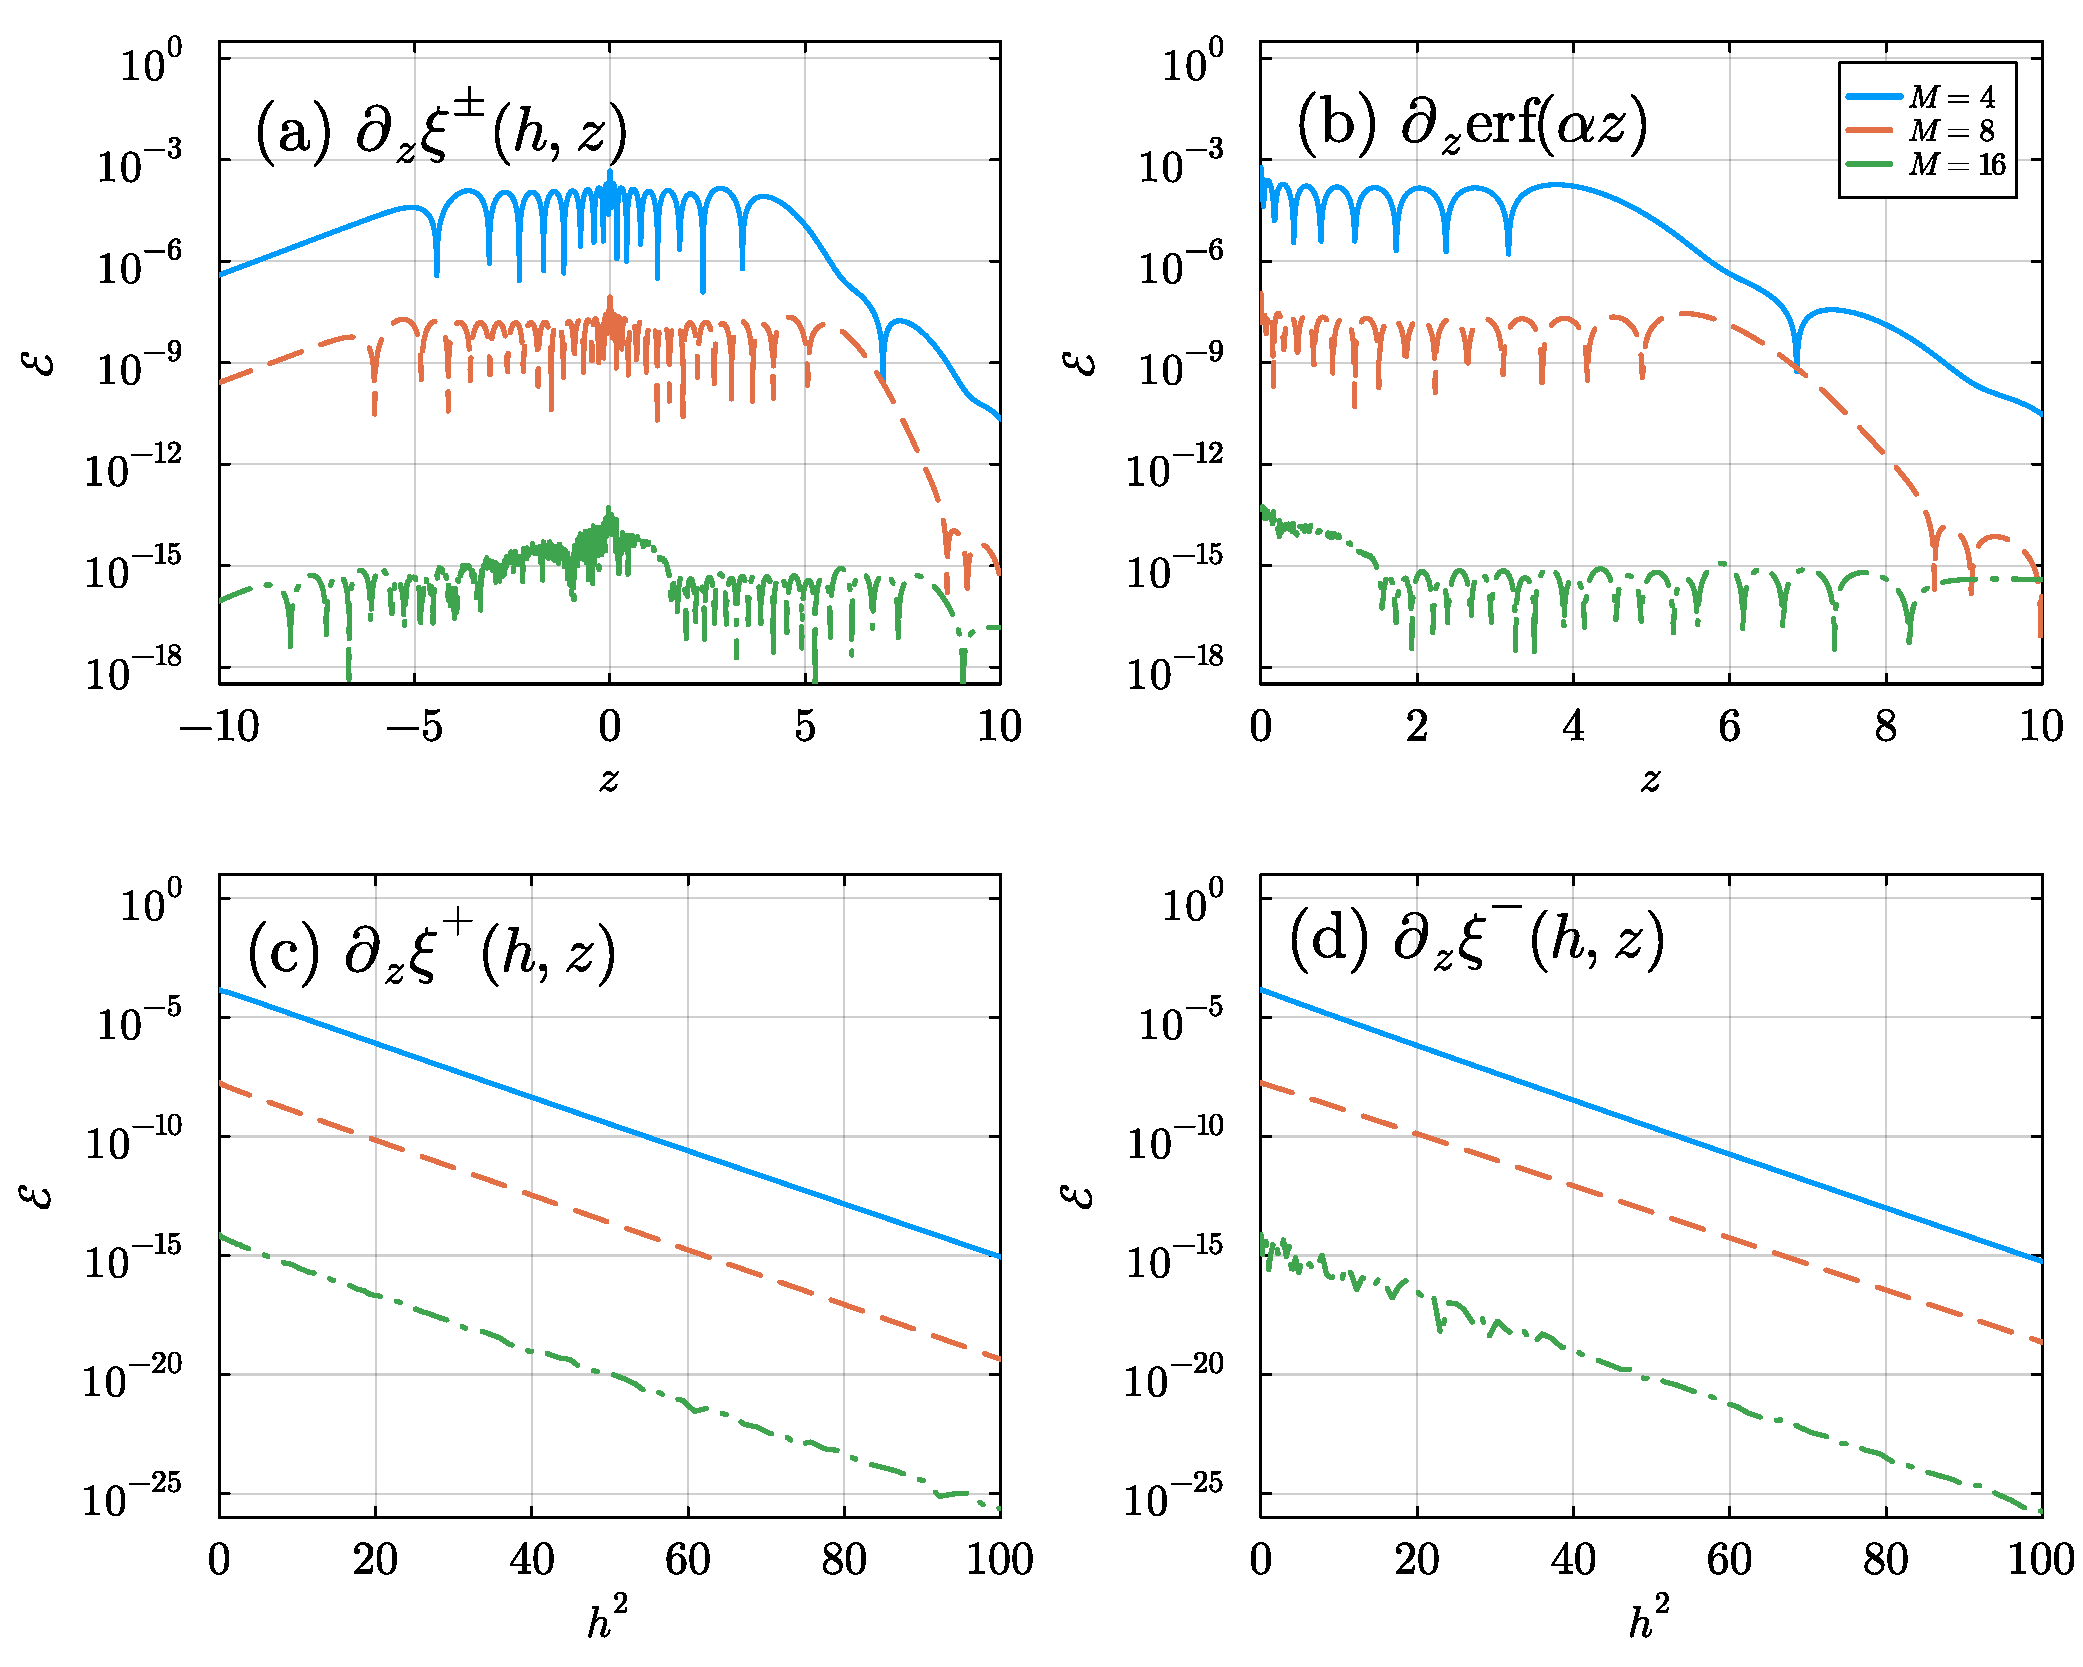
\includegraphics[width=\textwidth]{figs/fig_error_diff.pdf}
	%     \caption{
		%         The absolute error of the SOE expansion for (a) $\partial_z \xi^{\pm}(k,z)$ and (b) $\partial_z \erf(\alpha z)$ is plotted as a function of $z$, with both $k$ and $\alpha$ fixed at $1$; absolute error of the SOE expansion of (c) $\partial_z \xi^{+}(k,z)$ and (d) $\partial_z \xi^{-}(k,z)$ as a function of $k^2$, while keeping $z=1$.
		%         Data are presented for SOEs with varying numbers of exponentials.
		%         }
	%     \label{fig:error_diff}
	% \end{figure}

\section{Force expression of the SOEwald2D} \label{app::force}

The Fourier component of force acting on the $i$th particle can be evaluated by taking the gradient of the energy with respect to the particle's position vector $\bm{r}_{i}$,
\begin{equation}\label{eq::Fi}
	\V{F}_{\ell}^i  \approx \V{F}^{i}_{\text{l},\text{SOE}} = -\grad_{\V{r}_{i}} U_{\ell,\text{SOE}} =  -\sum_{\bm{k}\neq \bm{0}} \grad_{\V{r}_{i}}U_{\ell,\text{SOE}}^{\V{k}} -\grad_{\V{r}_{i}} U_{\ell,\text{SOE}}^{\V{0}}
\end{equation}
where
\begin{align}    
	\grad_{\V{r}_{i}}U_{\ell,\text{SOE}}^{\V{k}} &= - \frac{\pi q_{i}}{L_x L_y} \left[ \sum_{1 \leq j < i} q_{j} \grad_{\V{r}_{i}} \varphi_{\text{SOE}}^{\V{k}}(\V{r}_{i}, \V{r}_{j}) +  \sum_{i < j \leq N} q_{j} \grad_{\V{r}_{i}} \varphi_{\text{SOE}}^{\V{k}}(\V{r}_{j}, \V{r}_{i}) \right]\;,\\
	\grad_{\V{r}_{i}} U_{\ell,\text{SOE}}^{\V{0}} &= - \frac{2 \pi q_{i}}{L_x L_y} \left[ \sum_{1 \leq j < i} q_{j} \grad_{\V{r}_{i}} \varphi^{\bm{0}}_{\text{SOE}}(\bm{r}_{i}, \bm{r}_{j}) + \sum_{i < j \leq N} q_{j} \grad_{\V{r}_{i}} \varphi^{\bm{0}}_{\text{SOE}}(\bm{r}_{j}, \bm{r}_{i})\right]\;.
\end{align}
Using the approximation Eqs.~\eqref{eq::SOEphi},~\eqref{eq::dz_plus} and~\eqref{eq::dz_minus}, one can write the derivative in periodic directions as
\begin{equation}
	\begin{split}
		\partial_{\bm{\rho}_{i}} \varphi_{\text{SOE}}^{\V{k}}(\V{r}_{i}, \V{r}_{j}) & = \frac{\m{i} \V{k} e^{ \m{i} \V{k} \cdot \V{\rho}_{ij}}}{k} \left[\xi^{+}_M(k, z_{ij})+\xi^{-}_M(k, z_{ij})\right]\\
		&=\frac{2\alpha e^{-k^2/(4\alpha^2)}}{\sqrt{\pi}k} \m{i} \bm{k}e^{\m{i} \V{k} \cdot \V{\rho}_{ij}} \sum_{\ell = 1}^{M}  \frac{w_l}{\alpha^2 s_l^2 - k^2}\left( 2 \alpha s_l e^{-k z_{ij}} - 2 k e^{-\alpha s_l z_{ij}}\right),
	\end{split}
\end{equation}
and in~$z$ direction as
\begin{equation}\label{eq:z-der}
	\begin{split}
		\partial_{z_{i}} \varphi_{\text{SOE}}^{\V{k}}(\V{r}_{i}, \V{r}_{j}) & = \frac{e^{\m{i} \V{k} \cdot \V{\rho}_{ij}}}{k} \left[\partial_{z_{i}} \xi^{+}_M(k, z_{ij}) + \partial_{z_{i}} \xi^{-}_M(k, z_{ij})\right]\\
		&=\frac{2 \alpha e^{-k^2/(4\alpha^2)}}{\sqrt{\pi}}e^{ \m{i} \V{k} \cdot \V{\rho}_{ij}} \sum_{\ell = 1}^{M}  \frac{w_l}{\alpha^2 s_l^2 - k^2}\left( - 2 \alpha s_l e^{-k z_{ij}} + 2 \alpha s_l e^{- \alpha s_l z_{ij}}\right)\;.
	\end{split}
\end{equation}
The partial derivatives of zero-frequency mode with respect to the periodic directions are zero, and the SOE approximation of its $z$-derivative is given by
\begin{equation}\label{eq:dzphi_0}
	\begin{split}
		\partial_{z_{i}} \varphi^{\bm{0}}_{\text{SOE}}(\bm{r}_{i},\bm{r}_{j}) 
		& = \sum_{l=1}^{M} \frac{w_l}{\sqrt{\pi}} \partial_{z_{i}} \left[\frac{2z_{ij}}{s_l}+\left(\frac{1}{\alpha} - \frac{2z_{ij}}{s_l}\right)e^{-\alpha s_l z_{ij}}\right] \\
		& = \sum_{l=1}^{M} \frac{w_l}{\sqrt{\pi}} \left[ \frac{2}{s_l} - \left( s_l + \frac{2}{s_l} - 2 \alpha z_{ij} \right) e^{-\alpha s_l z_{ij}} \right]\;.
	\end{split}
\end{equation}

It is important to note that the computation of Fourier space forces using Eq.~\eqref{eq::Fi} follows a common recursive procedure with energy, since it has the same structure as given in Eq.~\eqref{eq::33}, and the overall cost for evaluating force on all~$N$ particles for each~$k$ point also amounts to~$\mathcal{O}(N)$, and the resulting SOEwald2D method is summarized in Algorithm~\ref{alg:SOEwald2D}.

Moreover, Lemma~\ref{lem::forceerr} establishes the overall error on forces $\bm{F}_{i}$, and the proof follows an almost similar approach to what was done for the energy. %The proof is postponed to~\ref{app::forceerror}

\begin{lem}\label{lem::forceerr}
	The total error of force by the SOEwald2D is given by
	\begin{equation}
		\mathscr{E}_{\bm{F}_{i}} := \mathscr{E}_{\bm{F}_{\emph{s}}^{i}} + \mathscr{E}_{\bm{F}_{\emph{l}}^{i}} + \sum_{\bm{k}\neq \bm{0}} \mathscr{E}_{\bm{F}_{\emph{l}}^i, \emph{SOE}}^{\bm{k}} + \mathscr{E}_{\bm{F}_{\emph{l}}^{i},\emph{SOE}}^{\bm{0}}
	\end{equation}
	where the first two terms are the truncation error and provided in Proposition~\ref{prop::2.12}. The remainder terms 
	\begin{equation}
		\mathscr{E}_{\bm{F}_{\emph{l}}^i,\emph{SOE}}^{\bm{k}} := \bm{F}_{\emph{l}}^{\bm{k}, i} - \bm{F}_{\emph{l},\emph{SOE}}^{\bm{k}, i}, \quad\emph{and} \quad \mathscr{E}_{\bm{F}_{\emph{l}}^{i}, \emph{SOE}}^{\bm{0}} := \bm{F}_{\emph{l}}^{\bm{0}, i}-\bm{F}_{\emph{l}, \emph{SOE}}^{\bm{0}, i}
	\end{equation}
	are the error due to the SOE approximation as Eqs.~\eqref{eq::Fi}-\eqref{eq:z-der}. Given SOE parameters $w_l$ and $s_l$ along with the ideal-gas assumption, one has the following estimate:
	\begin{equation}
		\sum_{\bm{k}\neq\bm{0}} \mathscr{E}_{\bm{F}_{\emph{l}}^i, \emph{SOE}}^{ \bm{k}}\leq \sqrt{2}\lambda_D^2\alpha^2q_{i}^2\varepsilon,\quad\text{and}\quad \mathscr{E}_{\bm{F}_{\emph{l}}^{i},\emph{SOE}}^{\bm{0}}\leq \frac{4\sqrt{\pi}\lambda_D^2 (1+2\alpha)L_z}{L_xL_y}q_{i}^2\varepsilon.
	\end{equation}
\end{lem}

\section{The Debye-H$\ddot{\text{u}}$ckel approximation}\label{app::Debye}
Under the DH approximation, one is able to estimate functions associated with the $i$-th particle in the form:
\begin{equation}
	\mathscr{G}(\bm{r}_i)=\sum_{j\neq i}q_{j}e^{\m{i} \bm{k}\cdot\bm{\rho}_{ij}}f(z_{ij}),
\end{equation}
where $|f(z_{ij})|$ is bounded by a constant $C_f$ independent of $z_{ij}$. The DH theory considers the simplest model of an electrolyte solution confined to the simulation cell, where all $N$ ions are idealized as hard spheres of diameter $r_{a}$ carrying charge $\pm q$ at their centers. The charge neutrality condition requires that $N_+=N_-=N/2$. Let us fix one ion of charge $+q$ at the origin $r=0$ and consider the distribution of the other ions around it.

In the region $0<r\leq r_{a}$, the electrostatic potential $\phi(\bm{r})$ satisfies the Laplace equation $-\Delta\phi(\bm{r})=0$. For $r\geq r_{a}$, the charge density of each species is described by the Boltzmann distribution $\rho_{\pm}(\bm{r})=\pm qe^{\mp\beta q\phi(\bm{r})}\rho_r/2$ with number density $\rho_r=N/V$. In this region, the electrostatic potential satisfies the linearized Poisson-Boltzmann equation~\cite{levin2002electrostatic}:
\begin{equation}
	-\Delta \phi(\bm{r})=2\pi\left[q \rho_r e^{-\beta q\phi(\bm{r})}-q\rho_r e^{+\beta q\phi(\bm{r})}\right]\approx -4\pi \beta q^2\rho_r\phi(\bm{r}),
\end{equation}
and its solution is given by
\begin{equation}
	\phi(\bm{r})=\begin{cases}
		\dfrac{q}{4\pi r}-\dfrac{q\kappa}{4\pi (1+\kappa a)},& r<r_{a},\\[1em]
		\dfrac{qe^{\kappa a}e^{-\kappa r}}{4\pi r(1+\kappa a)},&r\geq r_{a},
	\end{cases}
\end{equation}
where $\kappa=\sqrt{\beta q^2\rho}$ denotes the inverse of Debye length $\lambda_{\text{D}}$. By this definition, the net charge density for $r>r_{a}$ is $\rho_>(\bm{r})=-\kappa^2\phi(\bm{r})$. Let us fix $\bm{r}_i$ at the origin. Given these considerations, for $r\geq r_a$, one obtains the following estimate:
\begin{equation}\label{eq::E.4}
	\begin{split}
		|\mathscr{G}(\bm{r}_i)|&\approx \left|\int_{\mathbb{R}^3\backslash B(\bm{r}_{i}, r_a)}\rho_>(\bm{r})e^{-\m{i} \bm{k}\cdot\bm{\rho}}f(z)d\bm{r}\right|\\
		&\leq \frac{q_iC_fe^{\kappa a}}{4\pi(1+\kappa a)}\int_{a}^{\infty}\frac{e^{-\kappa r}}{r}4\pi r^2dr\\
		&=q_iC_f\lambda_{\text{D}}^2.
	\end{split}
\end{equation}

It is remarked that upper bound Eq.~\eqref{eq::E.4} is derived under the continuum approximation. In the presence of surface charges, the charge distribution along the $z$-direction may lack spatial uniformity. However, due to the confinement of particle distribution between two parallel plates, the integral in Eq.~\eqref{eq::E.4} along the $z$-direction remains bounded. An upper bound in the form of $|\mathscr{G}(\bm{r}_i)|\leq C_s C_{f}q_i$ can still be expected, where $C_s$ is a constant related to the thermodynamic properties of the system.

%the electrostatic potential satisfies the Poisson's equation
%\begin{equation}
%-\Delta \phi(\bm{r})=4\pi \rho_{q}(\bm{r}),\quad\rho_{q}(\bm{{r}})=q\rho_+g_{++}(\bm{r})-q\rho_{-}g_{+-}(\bm{r}),
%\end{equation}
%where the charge density are expressed in terms of the charge-charge correlation functions $g_{++}(\bm{r})=g_{--}(\bm{r})(\bm{r})$ and $g_{+-}(\bm{r})=g_{-+}(\bm{r})$, and $\rho_+=\rho_-=\rho/2$ are average densities of positive and negative ions. In the work of Debye and H$\ddot{\text{u}}$ckel, the correlation functions are approximated by $g_{ij}(\bm{r})=e^{-\beta q_j\phi_i(\bm{r})}$, 

%\section{The SOE approximation error of force}\label{app::forceerror}

\section{The Metropolis algorithm} \label{app::Metropolis}

In practice, the Metropolis algorithm~\cite{metropolis1953equation, hastings1970monte} is employed to generate a sequence $\{\bm{k}_{\eta}\}_{\eta=1}^{P}$ from $h(\bm{k})$. 
Since $\bm{k}\circ \bm{L}=2\pi \bm{m}$ with $\bm{m}$ an integer vector, one can conveniently sample from the discrete distribution $\mathcal{H}(\bm{m})=h(\bm{k})$ to equivalently generate $\bm{k}$. 
Once the current state of the Markov chain $\bm{m}_{\eta}=\bm{m}^{\text{old}}$ is known, the algorithm generates a random variable $\bm{m}^*$ with $m_{\xi}^*\sim \mathcal{N}[0,(\alpha L_{\xi})^2/2\pi^2]$, which is the normal distribution with mean zero and variance $(\alpha L_{\xi})^2/2\pi^2$. The new proposal is taken as $\bm{m}^{\text{new}}=\text{round}(m_{x}^*,m_{y}^*)$. To determine the acceptance rate, one obtains the proposal probability 
\begin{equation}
	q(\bm{m}^{\text{new}}|\bm{m}^{\text{old}})=\prod_{\xi\in\{x,y\}}q(m^{\text{new}}_{\xi}|m^{\text{old}}_{\xi})
\end{equation}
where
\begin{equation}
	\begin{split}
		q(m^{\text{new}}_{\xi}|m^{\text{old}}_{\xi})&=\sqrt{\frac{\pi}{(\alpha L_{\xi})^2}}\int_{m^{\text{new}}_{\xi}-\frac{1}{2}}^{m^{\text{new}}_{\xi}+\frac{1}{2}}e^{-\pi^2t^2/(\alpha L_{\xi})^2}dt\\[1em]
		&=\begin{cases}
			\erf\left(\dfrac{\pi}{2\alpha L_{\xi}}\right),&m_{\xi}^{\text{new}}=0,\\[1.15em]
			\dfrac{1}{2}\left[\erf\left(\dfrac{\pi(2|m_{\xi}^{\text{new}}|+1)}{2\alpha L_{\xi}}\right)-\erf\left(\dfrac{\pi(2|m_{\xi}^{\text{new}}|-1)}{2\alpha L_{\xi}}\right)\right],&m_{\xi}^{\text{new}}\neq 0.
		\end{cases}
	\end{split}
\end{equation}
It is worth noting that the proposal distribution $q(\bm{m}^{\text{new}}|\bm{m}^{\text{old}})$ in the Metropolis algorithm presented here does not depend on the current state $\bm{m}^{\text{old}}$. The Metropolis acceptance probability is computed using the formula:
\begin{equation}
	a(\bm{m}^{\text{new}}|\bm{m}^{\text{old}}):=\min\left\{\frac{\mathcal{H}(\bm{m}^{\text{new}})q(\bm{m}^{\text{old}}|\bm{m}^{\text{new}})}{\mathcal{H}(\bm{m}^{\text{old}})q(\bm{m}^{\text{new}}|\bm{m}^{\text{old}})},1\right\}.
\end{equation}
If the proposal is rejected, then $\bm{m}_{\eta+1}=\bm{m}_{\eta}$. If $\bm{m}^{\text{new}}$ is accepted, then $\bm{m}_{\eta+1}=\bm{m}^{\text{new}}$. The sampling procedure has a small error since $\mathcal{H}(\bm{m}^{\text{new}})\approx q(\bm{m}^{\text{new}}|\bm{m}^{\text{old}})$. Our numerical experiments show an average acceptance rate of over $90\%$. Additionally, one can set an integer downsampling rate $\mathscr{D}$, where only one sample is taken from every $\mathscr{D}$ samples, to reduce the correlation between batches in the Metropolis process.